\documentclass[12pt]{article}
%\topmargin=-0.5in
%\textheight=9in
%\evensidemargin=0in
%\oddsidemargin=0in
%\setlength{\textwidth}{6.5in}

% Replace "Thesis Title", "Student name" etc. below with the correct values
% These values will then be automatically added wherever necessary in thesis-template.tex and defence-announcement.tex

\newcommand{\thesistitle}{Multilingual Digital Signage using Computer Vision and Bluetooth Beacons}
\newcommand{\studentname}{Suhas Dwarakanath}
\newcommand{\advisorname}{Dr. Brian Thoms}

% Custom commands for other often used strings (\pythonversion, \submissionyear etc.) can be added
% below using the following template
% \newcommand{\<commandname>}{<commandvalue>} 

\usepackage{amsmath,latexsym}
\usepackage{amsfonts}
\usepackage{amssymb}
\usepackage{amssymb}
\usepackage{graphicx}
%\usepackage{appendix}
%\usepackage{clrscode3e}
\usepackage{epstopdf}
\usepackage{subfigure}
%\usepackage{algorithm}
%\usepackage{algorithmic}
\usepackage{setspace}
\usepackage{color}
\usepackage{listings}
\usepackage{setspace}
\usepackage{algpseudocode}
\usepackage{algorithm}
\usepackage[all]{xy}
\usepackage{pdfpages}
\usepackage{titlesec}

% Ensures a new section is on its own page. Must be done before hyperref is loaded

%changed by Suhas

 \newcommand{\sectionbreak}{\clearpage}

% Clickable references
\usepackage[hidelinks]{hyperref}

% Ensures graphic is in view after clicking on a reference to see it
\usepackage[all]{hypcap} 


% \doublespacing
\renewcommand{\topfraction}{0.9}	% max fraction of floats at top
\renewcommand{\bottomfraction}{0.8}	% max fraction of floats at bottom

%   Parameters for TEXT pages (not float pages):
\setcounter{topnumber}{2}
\setcounter{bottomnumber}{2}
\setcounter{totalnumber}{4}      % 2 may work better
\setcounter{dbltopnumber}{2}    % for 2-column pages
\renewcommand{\dbltopfraction}{0.9}	% fit big float above 2-col. text
\renewcommand{\textfraction}{0.07}	% allow minimal text w. figs

%   Parameters for FLOAT pages (not text pages):
\renewcommand{\floatpagefraction}{0.7}	% require fuller float pages
    
% N.B.: floatpagefraction MUST be less than topfraction !!
\renewcommand{\dblfloatpagefraction}{0.7}	% require fuller float pages

\newenvironment{dig}{\\ [6pt]\noindent {\bf Digression}}{~$\Box$\\ [6pt]\indent}
\newenvironment{dig1}{\noindent {\bf Digression}}{~$\Box$\\ [6pt]\indent}
\newtheorem{alg}{\hspace{1.3in} Algorithm}
\newtheorem{thrm}{Theorem}
\newtheorem{lemm}[thrm]{Lemma}
\newtheorem{conj}[thrm]{Conjecture}
%\newtheorem{claim}[thrm]{Claim}
\newtheorem{prop}[thrm]{Proposition}
\newtheorem{defn}[thrm]{Definition}
\newtheorem{obs}[thrm]{Observation}

\hyphenation{Chris-to-dou-lak-is}
\def\proof{\bigbreak\noindent {\sl Proof.\/}\enspace}
\def\qedbox#1#2{\vbox{\hrule height.2pt
  \hbox{\vrule width.2pt height#2pt \kern#1pt \vrule width.2pt}
  \hrule height.2pt}}
\def\qed{\hfill \quad\qedbox46\newline\smallbreak}

\def\s#1{\mbox{\boldmath $#1$}}
\def\floor#1{\lfloor #1 \rfloor}
\def\bfloor#1{\big\lfloor #1 \big\rfloor}
\def\Bfloor#1{\Big\lfloor #1 \Big\rfloor}
\def\ceil#1{\lceil #1 \rceil}
\def\bceil#1{\big\lceil #1 \big\rceil}
\def\+{\!+\!}
\def\-{\!-\!}
\def\plmi{\!\pm\!}
\def\m{\!-\!}
\def\uu#1{\underline{#1}}
\def\o#1{\overline{#1}}
\def\itbf#1{\textit{\textbf{#1}}}
\def\match{\approx}
\def\cP{\mathcal{P}}
\def\G{\mathcal{G}}
\def\B{\mathcal{B}}
\def\O{\mathcal{O}}

\def\bproc{{\bf procedure\ }}
\def\bfunc{{\bf function\ }}
\def\bvar{{\bf var\ }}
\def\barray{{\bf array\ }}
\def\bof{{\bf of\ }}
\def\bfor{{\bf for\ }}
\def\bnull{{\bf null\ }}
\def\bto{{\bf to\ }}
\def\bdownto{{\bf downto\ }}
\def\bwhile{{\bf while\ }}
\def\brep{{\bf repeat\ }}
\def\buntil{{\bf until\ }}
\def\band{{\bf and\ }}
\def\bor{{\bf or\ }}
\def\bdo{{\bf do\ }}
\def\bif{{\bf if\ }}
\def\bthen{{\bf then\ }}
\def\belse{{\bf else\ }}
\def\belsif{{\bf elsif\ }}
\def\bnot{{\bf not\ }}
\def\bgoto{{\bf goto\ }}
\def\bcontinue{{\bf continue\ }}
\def\breturn{{\bf return\ }}
\def\bbreak{{\bf break\ }}
\def\boutput{{\bf output}}
\def\la{\leftarrow}
\def\ra{\rightarrow}
\def\llra{\Leftrightarrow}
\def\q{\quad}
\def\qq{\qquad}
\def\com#1{{\bf $\triangleright$}\hspace{6pt}{\sl #1}}
\def\rem#1{\hspace{24pt}{\sl #1}}
\def\pref(#1,#2){$#1$ is a prefix of $#2$}
\def\suff(#1,#2){$#1$ is a suffix of $#2$}
\def\FIND{\mbox{FIND}}
\def\reg(#1,#2){$#2$ is $#1$-regular}
\def\notreg(#1,#2){$#2$ is not $#1$-regular}
\def\top{\tt{top}}
\def\pop{\tt{pop}}
\def\push{\tt{push}}
\def\true{\tt{true}}
\def\false{\tt{false}}
\def\UPDATE\_F{\tt{UPDATE\_F}}
\def\LEAST{\tt{LEAST}}
\def\MERGE{\tt{MERGE}}
\def\mec{\tt{mec}}
\def\MEC{\tt{MEC}}
\def\CMEC{\tt{CMEC}}
\def\MELC{\tt{MELC}}
\def\CMELC{\tt{CMELC}}
\def\MELS{\tt{MELS}}
\def\CMELS{\tt{CMELS}}
\def\MCNT{\tt{MaxCount}}
\def\CLEN{\tt{CorLen}}

% \def\B{\tt{B}}
\def\Q'{\tt{Q'}}
\def\CP{\tt{CP}}
\def\MNC{\tt{MNC}}
\def\PR{\tt{PR}}
\def\PRS{\tt{PRS}}
\def\CPR{\tt{CPR}}
% \def\POS{\tt{POS}}
\def\LEN{\tt{LEN}}
\newcommand{\dd}{\mathinner{\ldotp\ldotp}}

\newif\ifShow
\Showfalse
% MATH -----------------------------------------------------------
\newcommand{\norm}[1]{\left\Vert#1\right\Vert}
\newcommand{\abs}[1]{\left\vert#1\right\vert}
\newcommand{\set}[1]{\left\{#1\right\}}
\newcommand{\Real}{\mathbb R}
\newcommand{\eps}{\varepsilon}
\newcommand{\To}{\longrightarrow}
\newcommand{\BX}{\mathbf{B}(X)}
\newcommand{\A}{\mathcal{A}}
% Algorithm ------------------------------------------------------

\algnewcommand{\LineComment}[1]{\State \(\triangleright\) \normalfont{\sl #1}}
\algtext*{EndWhile}% l
\algtext*{EndIf}% Remove "end if" text
\algtext*{EndFor}% Remove "end for" text
\algtext*{EndFor}% Remove "end for" text
\algtext*{EndProcedure}% Remove "end procedure" text

% manifold
\newcommand{\F}{{F}}
\newcommand{\scF}{\F}
\newcommand{\X}{{X}}
\newcommand{\Fhat}{\widehat\F}
\newcommand{\scN}{{\EuScript N}}
\newcommand{\scL}{{\EuScript L}}
\newcommand{\PP}{\mathbb P}
\newcommand{\R}{\mathbb R}
\newcommand{\C}{\mathbb C}
% \newcommand{\CP}{\C\PP}
\newcommand{\CH}{\C{\mathrm H}}
\newcommand{\Lie}{{\mathcal L}}
\newcommand{\cpn} {\CP^n}
\newcommand{\chn} {\CH^n}
\newcommand{\cptwo} {\CP^2}
\newcommand{\chtwo} {\CH^2}
\newcommand{\chone} {\CH^1}
%\newcommand{\mean}{{\mathcal m}}
\newcommand{\mean}{{\mathbf m}}
%\def\({\left (}
\def\({\left(}
%\def\){\right )}
\def\){\right)}
\def\<{\langle}
\def\>{\rangle}
\def\a {\alpha}
\def\b {\beta}
\def\l {\lambda}

% Pfaffian systems
\newcommand{\CC}{{\EuScript C}}
\newcommand{\I}{{\mathcal I}}
\newcommand{\J}{{\EuScript J}}
\newcommand{\K}{{\mathcal K}}
\newcommand{\Khat}{\widehat{\K}}
\newcommand{\M}{{\mathcal M}}
\newcommand{\V}{\mathcal V}
\newcommand{\calS}{\mathcal S}

% differential forms
\newcommand{\w}{\omega}
\newcommand{\kh}{\hat\kappa}
\newcommand{\diff}{{\operatorname{diff}}}
% \newcommand{\alg}{{\operatorname{alg}}}

%maps
\newcommand{\fhat}{\hat{f}}

%open sets
\newcommand{\setU}{\EuScript U}
\newcommand{\Uhat}{\widehat{\setU}}

% vectors
\newcommand{\e}{\mathbf e}
\newcommand{\ehat}{\hat{\e}}
\newcommand{\bv}{\mathbf v}
\newcommand{\bx}{\mathbf x}
\newcommand{\bg}{\mathbf g}
\newcommand{\by}{\mathbf y}
\newcommand{\bw}{\mathbf w}
\newcommand{\bxi}{\mathbf\xi}
\newcommand{\bn}{\mathbf n}
\newcommand{\bz}{\mathbf z}

% complex variables
\newcommand{\ri}{\mathrm i}
\newcommand{\realpart}{\operatorname{Re}}

% operators
\newcommand{\JJ}{{\mathrm J}} % complex structure
\newcommand{\RR}{{\sf R}} % curvature operator
\newcommand{\Ric}{{\sf Ric}} % Ricci tensor
\newcommand{\di}{\partial}
\newcommand{\dib}[1]{\di_{#1}}
\newcommand{\tvec}{\tfrac{\di}{\di t}}
\newcommand{\restr}{\negthickspace \mid}
\newcommand{\transpose}[1]{{}^t\hskip-2pt{#1}}
\newcommand{\nat}{\widetilde\nabla}
\newcommand{\RRt}{\widetilde R}
\newcommand{\mt}{\widetilde M}
\def\intprod{\mathbin{\raisebox{.4ex}{\hbox{\vrule height .5pt width
5pt depth 0pt %
         \vrule height 3pt width .5pt depth 0pt}}}}
\newcommand{\hook}{\intprod}
\def\&{\wedge}
% \def\s{\sigma}
\def\a{\alpha}
\def\b{\beta}
\def\n{\nabla}

\title{\thesistitle} 
\author{\studentname}
\date{\today}

\begin{document}

\begin{titlepage}
\pagenumbering{gobble}
\begin{center}
{\Large \bfseries \thesistitle \par}

\vspace{2 cm}
\baselineskip = 2\baselineskip
A Thesis Presented to \\
The Faculty of the Computer Science Department\\
California State University Channel Islands

\vspace{1 cm}

In (Partial) Fulfillment\\
of the Requirements for the Degree\\
Masters of Science in Computer Science\\

\vspace{1 cm }

\vfill

by \\
\studentname\\
Advisor: \advisorname\\
March 2019
\end{center}
\end{titlepage}
\baselineskip = \baselineskip
\newpage

\null
\vfill
\begin{flushleft}
\copyright\; 2019\\
\studentname\\
ALL RIGHTS RESERVED
\end{flushleft}
\newpage

\begin{center}
{\large \bfseries APPROVED FOR MS IN COMPUTER SCIENCE \par}

\vspace{1.5 cm}

\hrulefill\\
{\large \bfseries Advisor: \advisorname \hfill Date \par}

\vspace{1.5 cm}

\hrulefill\\
{\large \bfseries Name \hfill Date \par}

\vspace{1.5 cm}

\hrulefill\\
{\large \bfseries Name \hfill Date \par}

\vspace{3 cm}

{\large \bfseries APPROVED FOR THE UNIVERITY \par}

\vspace{1.5 cm}

\hrulefill\\
{\large \bfseries Name \hfill Date \par}
\end{center}
\newpage

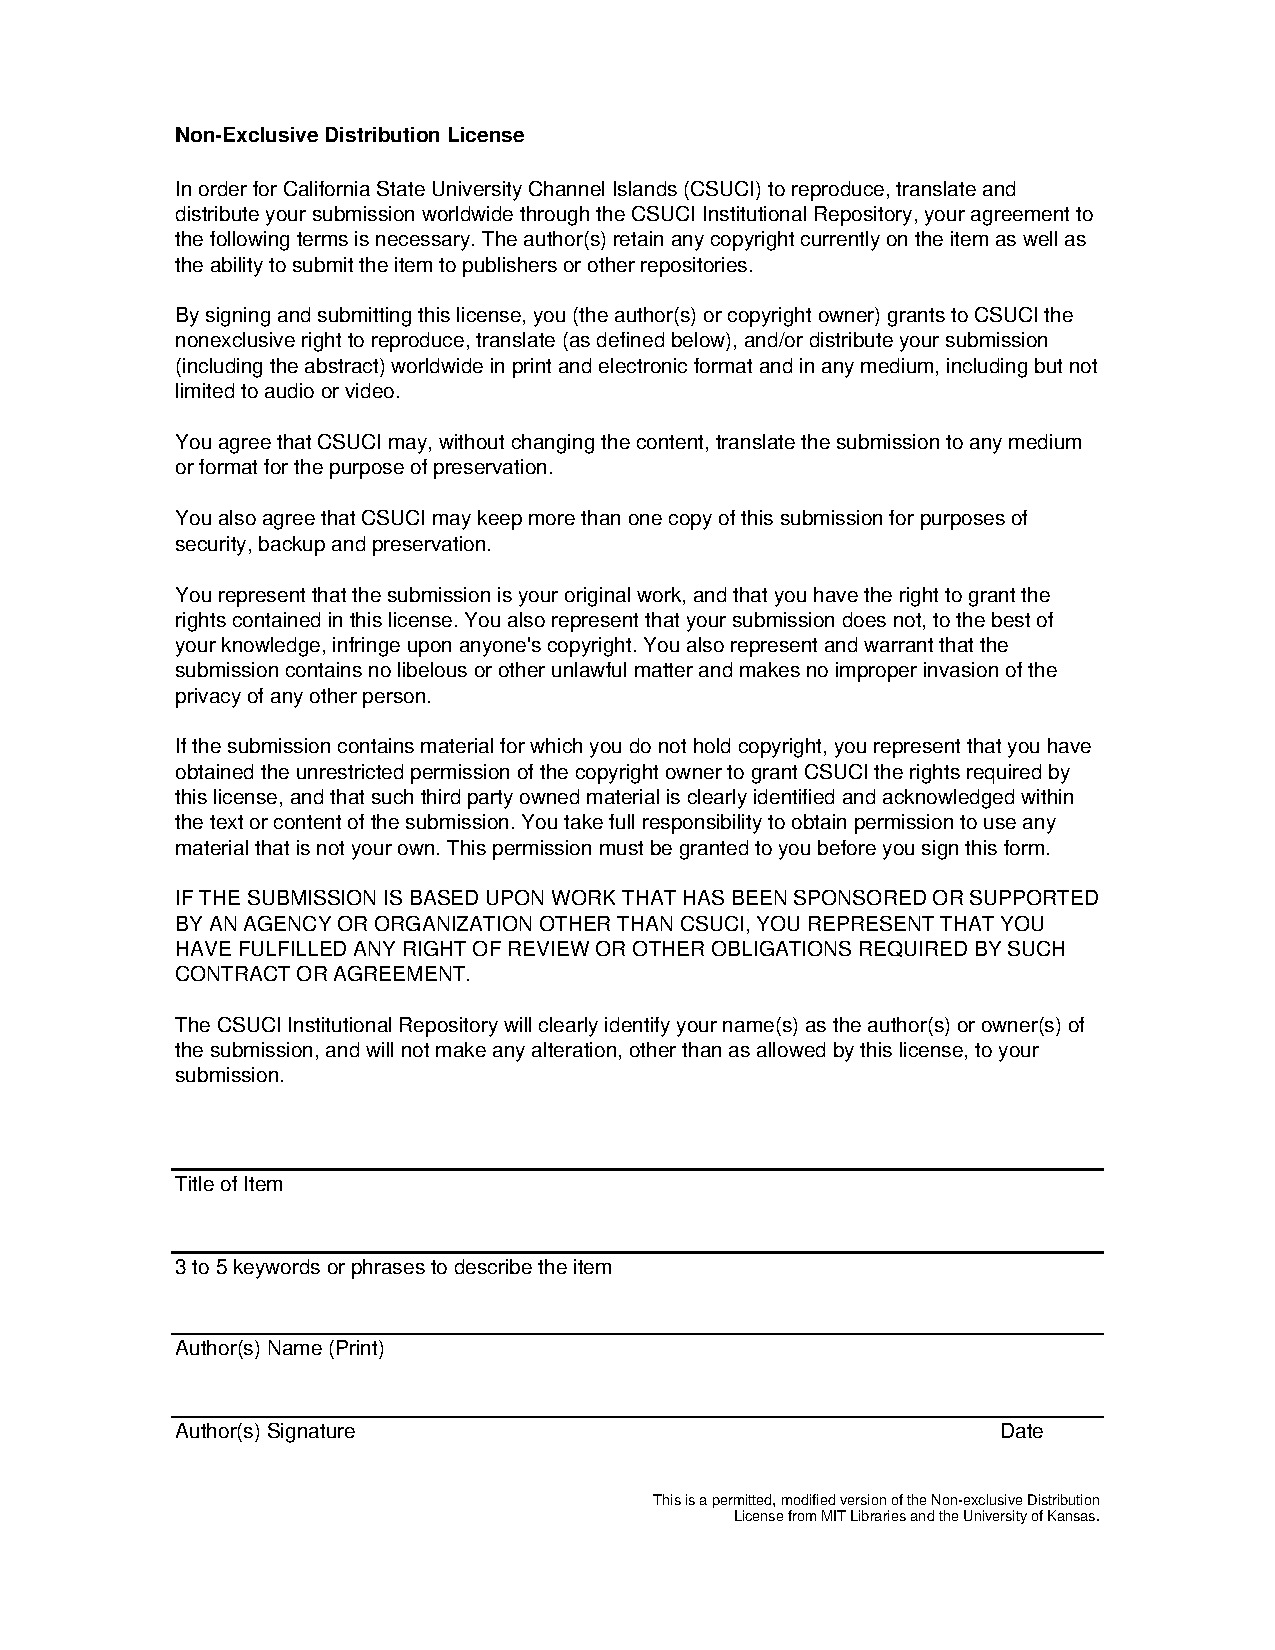
\includepdf{media/distribution-license.pdf}
\newpage


\maketitle

\begin{abstract}
Due to globalization and changing lifestyle, more and more people are visiting foreign countries for business and travel. Also lately, a lot of newly arriving refugee families to the U.S face legal consequences. One of the struggles they face is reading documentation they receive through mail; whether bills, court documents or financial assistance documents, they struggle to read and understand them. There are thousands of languages in the world and it is impractical to install signage and print documents in all the languages. In this research, by combining Computer Vision and Bluetooth beacons, multilingual digital information is displayed on the user's smartphone. Smartphone camera allows the user to take a picture of a document. It is then posted to the Google Cloud Vision API which returns the text of that document. It can then be translated to any language using Google Translate API. The system also displays the information of nearby signages (with bluetooth beacons) on the smartphone. This system was implemented in the university campus and the evaluation experiment was conducted by on international students. It was found that the system helps the users to understand their environment better in their native language.
\end{abstract}

\newpage
\pagenumbering{roman}

\tableofcontents

\newpage

\listoffigures

\newpage
\pagenumbering{arabic}

\section{Introduction}
\label{sect-intro}

With changing lifestyle and globalization, more people visit foreign countries. Every country is working towards becoming tourism oriented to increase their economy. Most of the visitors use their smartphone to access information. However, when visiting foreign countries, most people face difficulties in obtaining information due to difference in language, which makes it an inconvenience to stay in foreign countries for a longer time.  \\

Recently, a lot of refugee and migrant families from all over the world faced a lot of struggles at the U.S immigrations. A lot of these refugees faced problems with the documentation because they could not understand the content of the legal documents. It is natural for people to understand information better in their home language. Therefore, an effective method of providing and accessing information in multiple languages is required. \\

In this study, in order to solve such problems, a multilingual information service was developed using Computer Vision and Bluetooth beacons. The information can be accessed from the user's smartphone in most of the languages. We focus on the smartphone's camera to 'see' information in multiple languages. We also use bluetooth beacons to 'push' information to smartphones in proximity. The user can then access the information in multiple languages. By using this method, we expect people visiting foreign countries to access information naturally in the same way they would in their home countries. This paper evaluates various options like GPS, NFC and RFID which could be used to provide information based on user's location. We then describe the required functions and configuration of the prototype system developed. \\

An example citation: \cite{graves-1995}.\\

An example citation: \cite{one}.\\
%An example reference: \autoref{fig:ci-logo} (Notice references and citations are clickable!)

% When including grapics, make sure the directory is relative to root .tex document, not the current .tex file

%\begin{figure}[H]
%	\centering
%	
\includegraphics[width=0.7\linewidth]{media/ci-logo}
%	\caption{This is an example graphic}
%	\label{fig:ci-logo}
%\end{figure} 

\section{Background}
\label{sect-background}

\paragraph{}Text is highly researched area in the computer vision application to model a smart self-learning system, which involve text associated with shop banners, highway and roadside sign boards or the text on local transport system, such a text provide significant clues about that environment. Text detection helps visually impaired and tourist to convey correct information in more understandable way to user.

\paragraph{}As a method of accessing information on public signages, there are two ways of using a smart phone to find information in relevant languages; the user needs to search information by himself, then translate it relevant language to access necessary information. On the other hand, when the digital signage is used, the user can find and acquire information by walking in front of the digital signage without performing any special action. In this study, we explore ways to improve searching and accessing information by using smartphone camera and the method of information provision using the digital signage using iBeacons. This should make users who visit foreign countries get information without making special efforts. 

\subsection{Related Work}

\paragraph{} A study of multilingual digital signage using iBeacon communication was done, for the purpose of evaluating the technology in an university campus at Japan.  \cite{one} In the experiment, the authors installed a total of 25 iBeacon devices at some sightseeing spots, restaurants, souvenir shops, photo shops, etc. in Shirakawa-go, Japan. When vistors look at these heritage spots from the outside, it is difficult for them to understand whether it is a restaurant or a souvenir shop. By using this system, the tourists was able to obtain necessary information in their native languages when they enter each iBeacon area while walking in Shirakawa-go. The paper confirmed that this system can be used effectively for both Japanese and the foreigners \cite{one}.  In this system, it was possible to change the displayed language automatically when the user comes near to the digital signage, by using the mechanism of background communication of the iBeacon. \textbf{However, the study is dependent on installing and configuring bluetooth iBeacons for the user to be able to understand the signages.}

\paragraph{}In India, a study of text detection and extraction based on Stroke Width Transform (SWT) and methodology to extract letters was conducted. \cite{india} Major application focus were tourism industry and local transport, to help people to deal with different Indian languages which involve text associated with natural scenes in the local public places. Using SWT method, various Indian languages and their combination with English were detected. \textbf{However, this study does not translate the detected texts into the user's preferred languages. This is still a hindrance for foreigners to understand their environment.}

\paragraph{} The problem of proximity estimation is found to be difficult in a variety of environment. Existing approaches such as Global Positioning System and Wi-Fi triangulations are insufficient to meet the requirements of accuracy and also requires high cost. A study was made using, Bluetooth which is commonly available in all smartphones to find the proximity over a shorter distance and provide an estimation model to determine the distance based on the Received Signal Strength Indicator (RSSI) values of the Bluetooth  \cite{distance}. In existing system GPS is used to find the location, it won't work as accurately indoors and inside most commercial building areas. So the authors proposed a system to overcome the problem by using Bluetooth to Bluetooth proximity estimation. By using the signal strength of the Bluetooth device, estimated RSSI value is used to find out exact distance between the devices. This technique helps in tracking the location of nearby user. The study proposed the proximity estimation model by combining Bluetooth RSSI value. The results demonstrate that Bluetooth offers an effective mechanism that is accurate and power-efficient for measuring face-to-face proximity to increase Bluetooth signal length \cite{distance}. \textbf{While this study does not focus on text detection or digital signage, this is  useful for our study to determine the distance of the user/smartphone to the iBeacons} 

\paragraph{}Optical Character Recognition (OCR) is the electronic conversion of images into machine encoded text. It provides alphanumeric recognition of printed or handwritten characters. OCR has been an active topic of research in the recent past, and has wide applications in banking, healthcare, finance and education. According to the World Health Organization (WHO), around 285 million people around the world are estimated to be visually impaired, out of which 90\% live in developing countries. Thus there is a pressing need to develop a system to provide information to the visually impaired. The authors  proposed a camera based framework built on the Raspberry Pi, integrated with Image processing algorithms, OCR and Text-to-Speech (TTS) synthesis module \cite{ocr}. The camera module is used to capture an image of the printed text, and the image was then subject to preprocessing before being fed into the OCR.\cite{ocr} \textbf{This study, however does not focus on language translation or digital signage, we use the adopt image pre-processing techniques like binarization, de-noising, deskewing, segmentation and feature extraction in our research.}

\paragraph{}In Taiwan, to encourage learning English, a study was carried out using the iBeacon's micro-positioning function to set the location in museum, restaurant, store, etc. When your mobile phone detects the information of iBeacon's location situation, you can learn by interacting with users' surrounding environment. \cite{taiwan} English obtained from the vocabulary performance includes the single words and expressions commonly used in daily life. With the listing narration and use of straightforward sentence structure and grammar, users can learn English conveniently and rapidly and apply it flexibly to real situations. In this way, users can learn English whenever and wherever possible to enhance English ability, achieve better effects with half efforts and gain language learning fun in the proposed mobile application. With the combination of the proposed application, English learning materials and iBeacon micro-location feature, learners can receive the surrounding related learning materials. In this manner, learners will have chance to build the connection between the learning materials and the environment which can enforce their memory to remember the learning concept.  \cite{taiwan} It was found that the system can raise the learning intent of the learners and may improve their learning effectiveness. \textbf{However, this study focusses on converting Chinese language to English based on the user's location. It does not support multiple languages and the system is entirely dependent on iBeacons.}


\section{Conclusion and future work}
\label{sect-conclusion}
Your work goes here

\cleardoublepage
\phantomsection
\bibliographystyle{plain}
\bibliography{references}
\addcontentsline{toc}{section}{References}

\end{document}

